\section{Co-registered and geocoded SLC (CSLC \& GSLC)}
\label{sec:cslc_gslc}

\subsection{Evaluation criteria}
\label{sec:cslc_criteria}

The evaluation of \acs{cslc} products is primarily driven by the level of co-registration accuracy that can be achieved. Beyond this, the geometric and radiometric integrity of both \acs{cslc} and \acs{gslc} products should be verified against the original \acs{sar} imagery, ensuring that neither the co-registration nor the geocoding processes introduce any significant degradation to these essential image attributes.

Image co-registration refers to the alignment of two or more images such that each pixel corresponds to the same geographic location in the target scene. This process, which can achieve sub-pixel accuracy, is essential for the generation of consistent multidimensional image stacks and for enabling advanced analyses such as interferometry and time-series processing.

In the context of the \textit{ROSE-L} mission, co-registered products are provided in radar geometry \cite{RD41}. This product, known as the \acs{cslc} (Co-Registered Single-Look Complex), is fundamental for interferometric workflows. It includes corrections for geometric distortions (e.g., topographic effects), atmospheric delays (both tropospheric and ionospheric), and other influencing factors.

The \acs{cslc} retains the full fidelity of the original \acs{sar} data, without introducing distortions. The amplitude component corresponds to $\beta_{\mathrm{LUT}}^0$, derived during calibration from the beta-zero lookup table contained in the \acs{slc} annotations. The phase is flattened relative to the satellite orbit and a Digital Elevation Model (\acs{dem}).

To support analyses in map-projected (ground) geometry, \acs{slc} or \acs{cslc} products can be resampled onto a common geographic grid (e.g., \acs{utm}, \acs{ups}). The resulting product, referred to as the \acs{gslc} (Geocoded Single-Look Complex), improves usability—enabling direct visualisation in \acs{gis} environments and facilitating data fusion across multiple sensors. However, due to the interpolation and projection steps involved, the \acs{gslc} is less suitable for high-precision interferometric applications, such as coherence analysis or phase unwrapping.

Similar to the \acs{cslc}, the phase of the \acs{gslc} is flattened with respect to the orbit and the \acs{dem} to eliminate topographic contributions \cite{Zebker2017, Zheng2017}. The spatial resolution in map-projected coordinates is generally consistent with the native resolution of the original \acs{slc}.

A key requirement for both the \acs{cslc} and \acs{gslc} products is the preservation of the original radiometric and geometric properties of the \acs{sar} data.

To assess radiometric fidelity, a set of standard \acs{sar} image quality indicators will be used:

\begin{itemize}
    \item \textbf{Spatial Resolution}: Represents the sensor’s capacity to distinguish closely spaced features. It is typically assessed by examining the width of the impulse response from bright, isolated scatterers.
    \item \textbf{Integrated Side-Lobe Ratio (\acs{islr})}: Quantifies the ratio of energy in the side lobes to that in the main lobe of the point target response. Lower \acs{islr} values indicate reduced side-lobe energy and improved radiometric clarity.
    \item \textbf{Peak Side-Lobe Ratio (\acs{pslr})}: Denotes the ratio between the highest side-lobe peak and the main lobe. Lower \acs{pslr} values imply higher target separability and better contrast.
\end{itemize}

Any degradation in these indicators—observed after co-registration or geocoding—will provide insight into the impact of these processes on the radiometric quality of the resulting \acs{ard} products.

Geometric integrity is evaluated through the accuracy of co-registration and geolocation. This involves verifying that the spatial alignment of pixels remains within acceptable tolerances, particularly for applications demanding high positional accuracy.

These evaluations will be supported by the use of very bright and isolated point scatterers, such as corner reflectors, which serve as reliable references for both radiometric and geometric quality assessments.

\subsection{Theoretical models}
\label{sec:cslc_models}

\subsubsection{Co-registration accuracy}
\label{sec:cslc_coreg_geoloc}

Both the co-registration and geolocation processes rely on accurately identifying the radar image coordinates corresponding to known ground positions, typically derived from a Digital Elevation Model (\acs{dem}). In the case of co-registration, the points of DEM must be projected onto both the reference (master) and secondary (slave) \acs{sar} images. These projections are used to derive the spatial transformation required to resample the slave image onto the master image grid.

Similarly, in geocoding operations, each point on the target ground coordinate grid (e.g., in map-projected geometry) must be mapped back to its corresponding location in radar coordinates. The radiometric value at that radar position is then interpolated and assigned to the geocoded product. 

In both cases, the geometric accuracy of the final product is fundamentally determined by the precision with which radar coordinates can be retrieved for each ground coordinate. Consequently, any uncertainties in the orbital state vectors, DEM height accuracy, or any atmospheric delay directly propagates into co-registration and geolocation errors, affecting the overall geometric fidelity of the \acs{ard} products.

Uncertainties in orbit and \acs{dem} data introduce positional errors in both slant-range and azimuth directions. These errors can be analytically expressed as a function of satellite geometry and viewing parameters.

In particular, inaccuracies in orbit knowledge affect the ability to precisely reconstruct the slant-range and azimuth positions of each acquisition. 
A simplified sketch of the acquisition geometry is reported in Figure~\ref{fig:drg_from_dh}.

\begin{figure}[ht!]
\centering
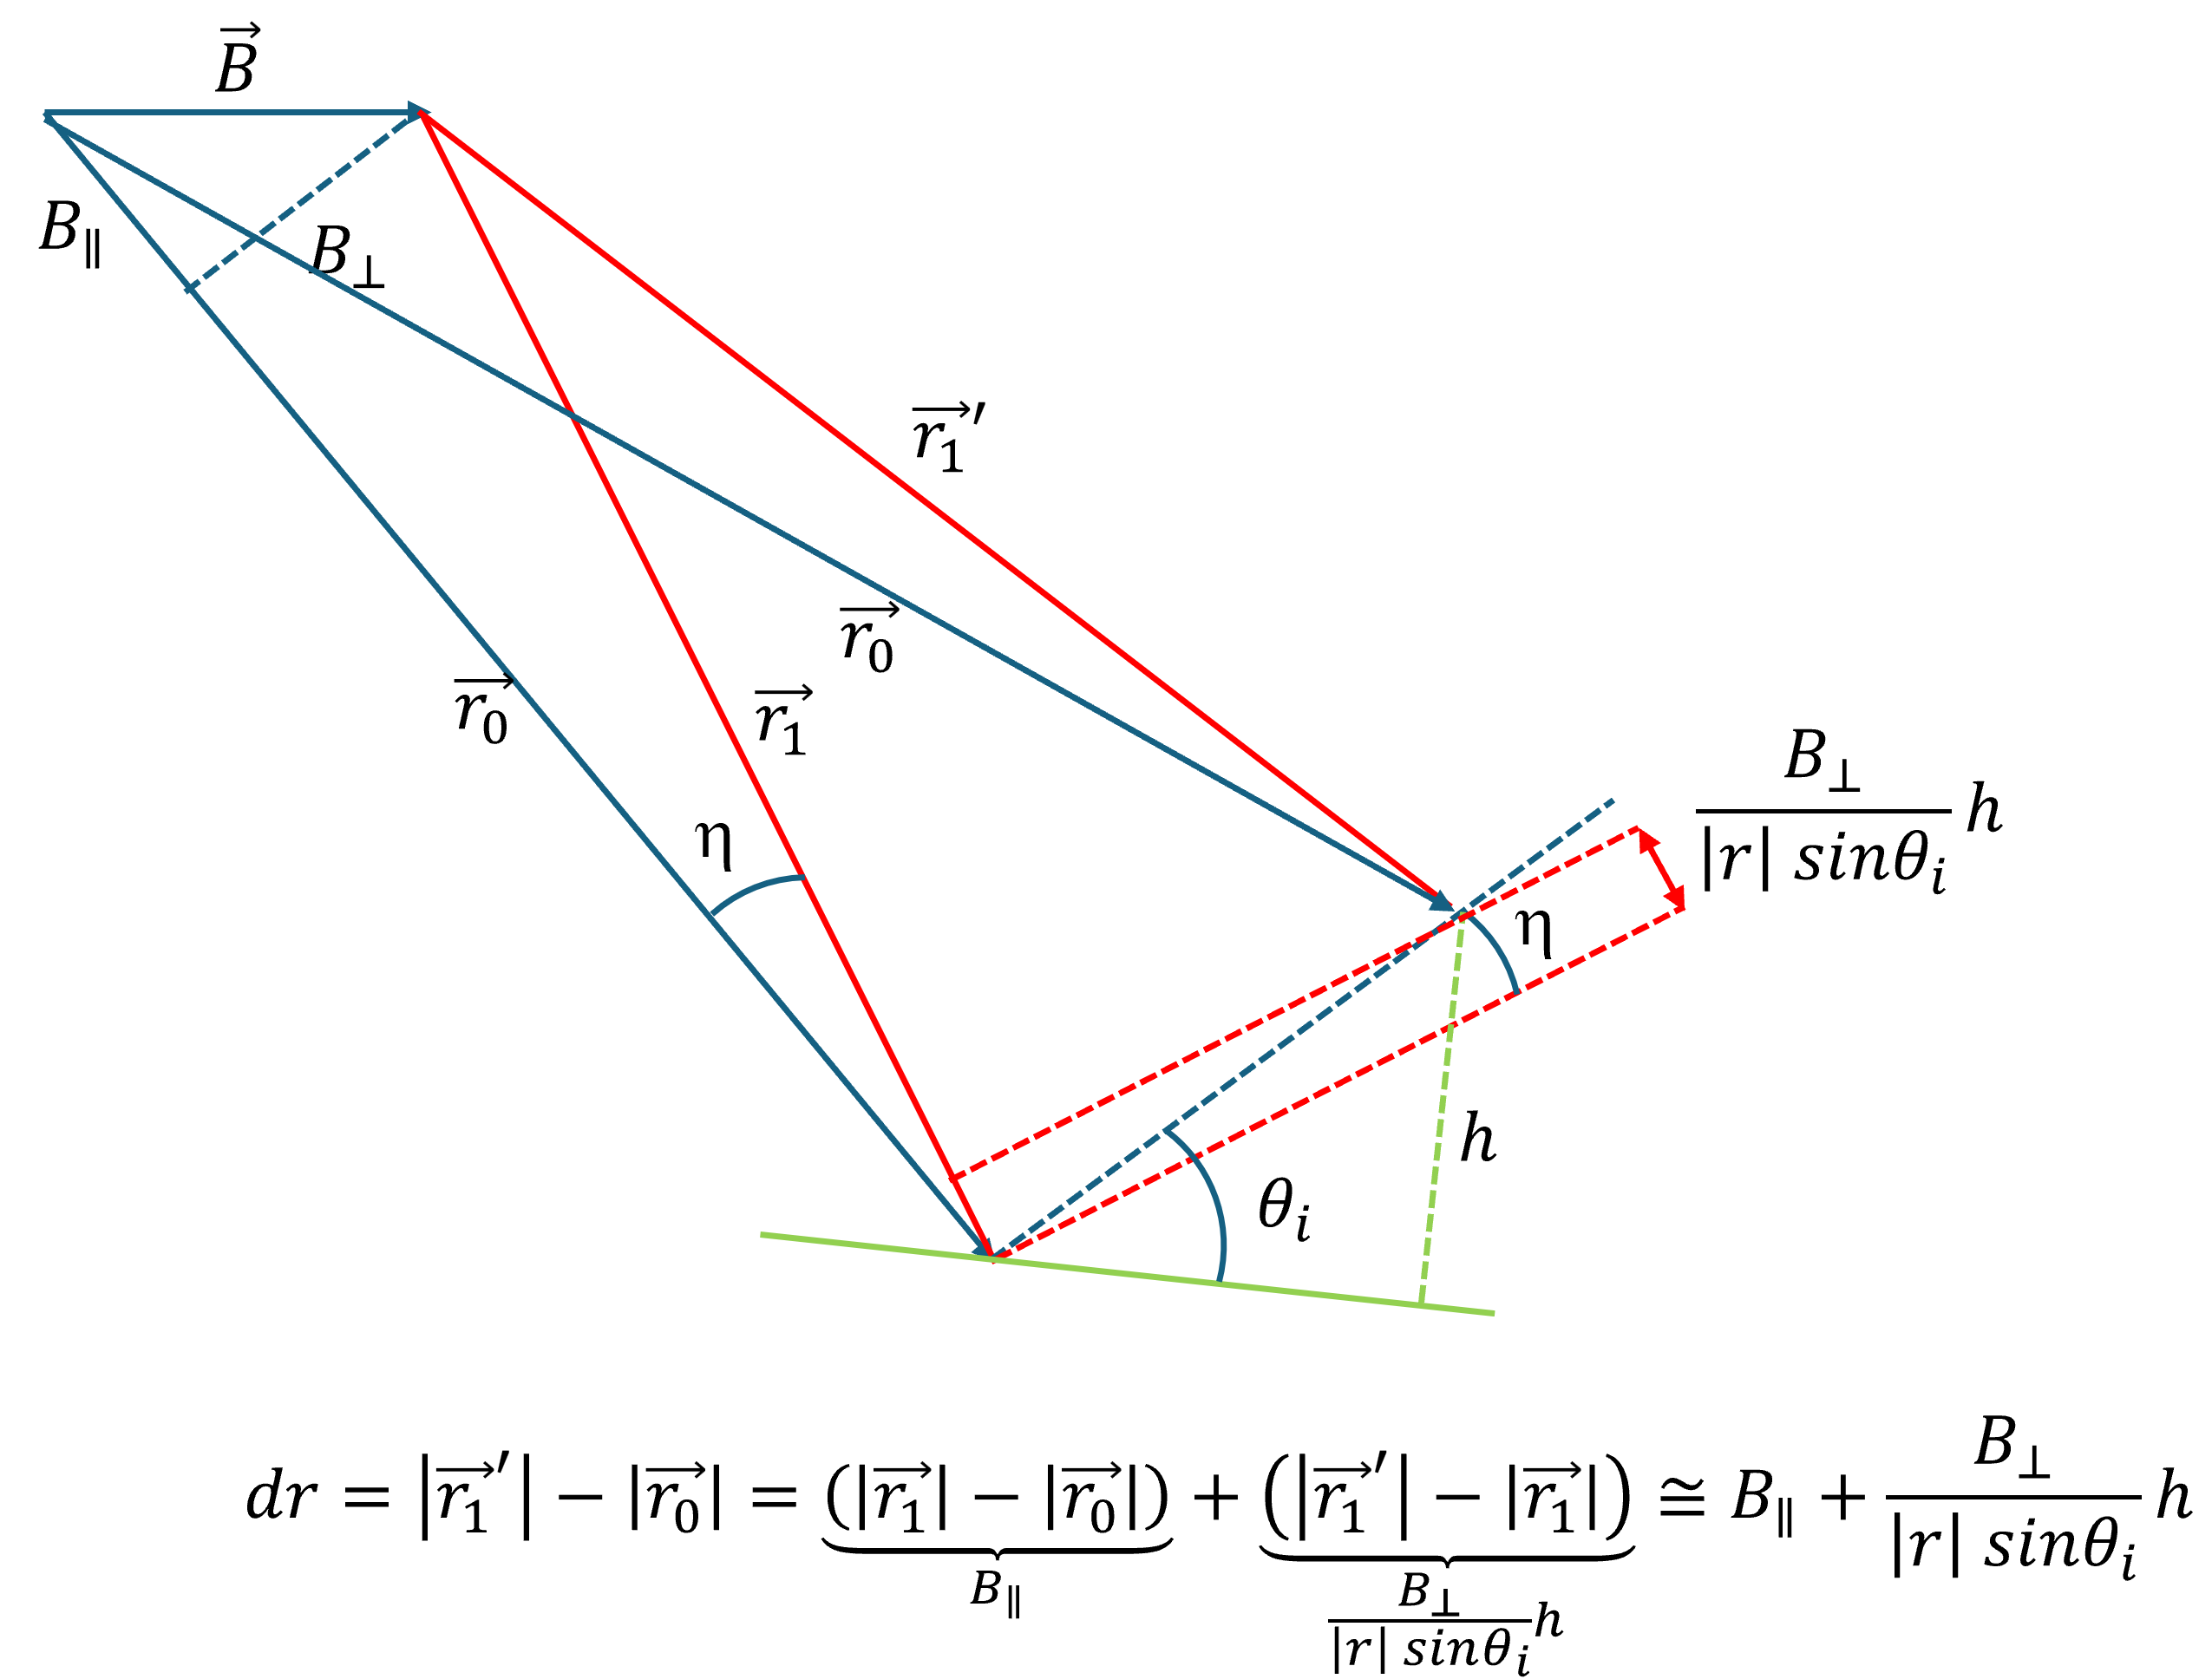
\includegraphics[width=0.9\textwidth]{Figures/cslc/dr_graph.png}
\caption{Simple sketch of the acquisition geometry. An error in the elevation of the target \(h\) implies an additional offset in range with respect to the difference in the satellite position in the line-of-sight of the reference image \(B_{\parallel}\).}
\label{fig:drg_from_dh}
\end{figure}

The standard deviation of the error in the slant-range position identification, denoted $\sigma_{dr}$, can be formulated as follows:

\begin{equation}
\sigma_{dr}^2 = \left(\frac{h}{R \sin\theta} \right)^2 \sigma_{B_{\perp}}^2 + \sigma_{B_{\parallel}}^2
\label{eq:slant_range_error_baseline}
\end{equation}

Here, $\sigma_{B_{\perp}}$ and $\sigma_{B_{\parallel}}$ represent the standard deviations of the perpendicular and parallel components, respectively, of the spatial baseline between the reference (master) and the secondary (slave) acquisition. The variables $h$, $R$, and $\theta$ correspond to the target height, slant-range distance, and incidence angle.

From equation~\ref{eq:slant_range_error_baseline}, it is evident that the first term is typically negligible in most scenarios. This is due to the fact that $h$ is generally on the order of a few kilometers, while $R \sin\theta$ is on the order of several hundred kilometers—thus significantly reducing the weight of the first term. Consequently, the dominant contribution to slant-range uncertainty is the uncertainty on the parallel component of the baseline, $\sigma_{B_{\parallel}}$.

This behavior is illustrated in Figure~\ref{fig:sigma_slant_range}, which shows the standard deviation in slant-range position $\sigma_{dr}$ (in meters) for various combinations of $(\sigma_{B_{\perp}}, \sigma_{B_{\parallel}}) \in \left[0, 0.25\right] \times \left[0, 0.25\right]$. As clearly shown, $\sigma_{dr}$ is most sensitive to variations in the parallel baseline uncertainty.

\begin{figure}[ht!]
\centering
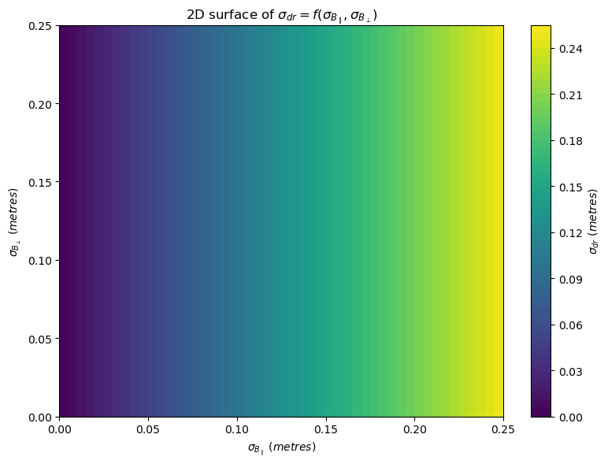
\includegraphics[width=0.9\textwidth]{Figures/cslc/sigma_slant_range.png}
\caption{Standard deviation in slant-range position $\sigma_{dr}$ (in meters) for each pair $(\sigma_{B_{\perp}}, \sigma_{B_{\parallel}}) \in \left[0, 0.25\right] \times \left[0, 0.25\right]$, assuming fixed parameters: $h = 1000$ m, $R = 600000$ m, and $\theta = 40^\circ$.}
\label{fig:sigma_slant_range}
\end{figure}

The error in azimuth position is determined by the zero-Doppler identification, which depends on the accuracy of the velocity vector. A simple sketch of the acquisition geometry is reported in Figure~\ref{fig:da_from_dv}.

\begin{figure}[ht!]
\centering
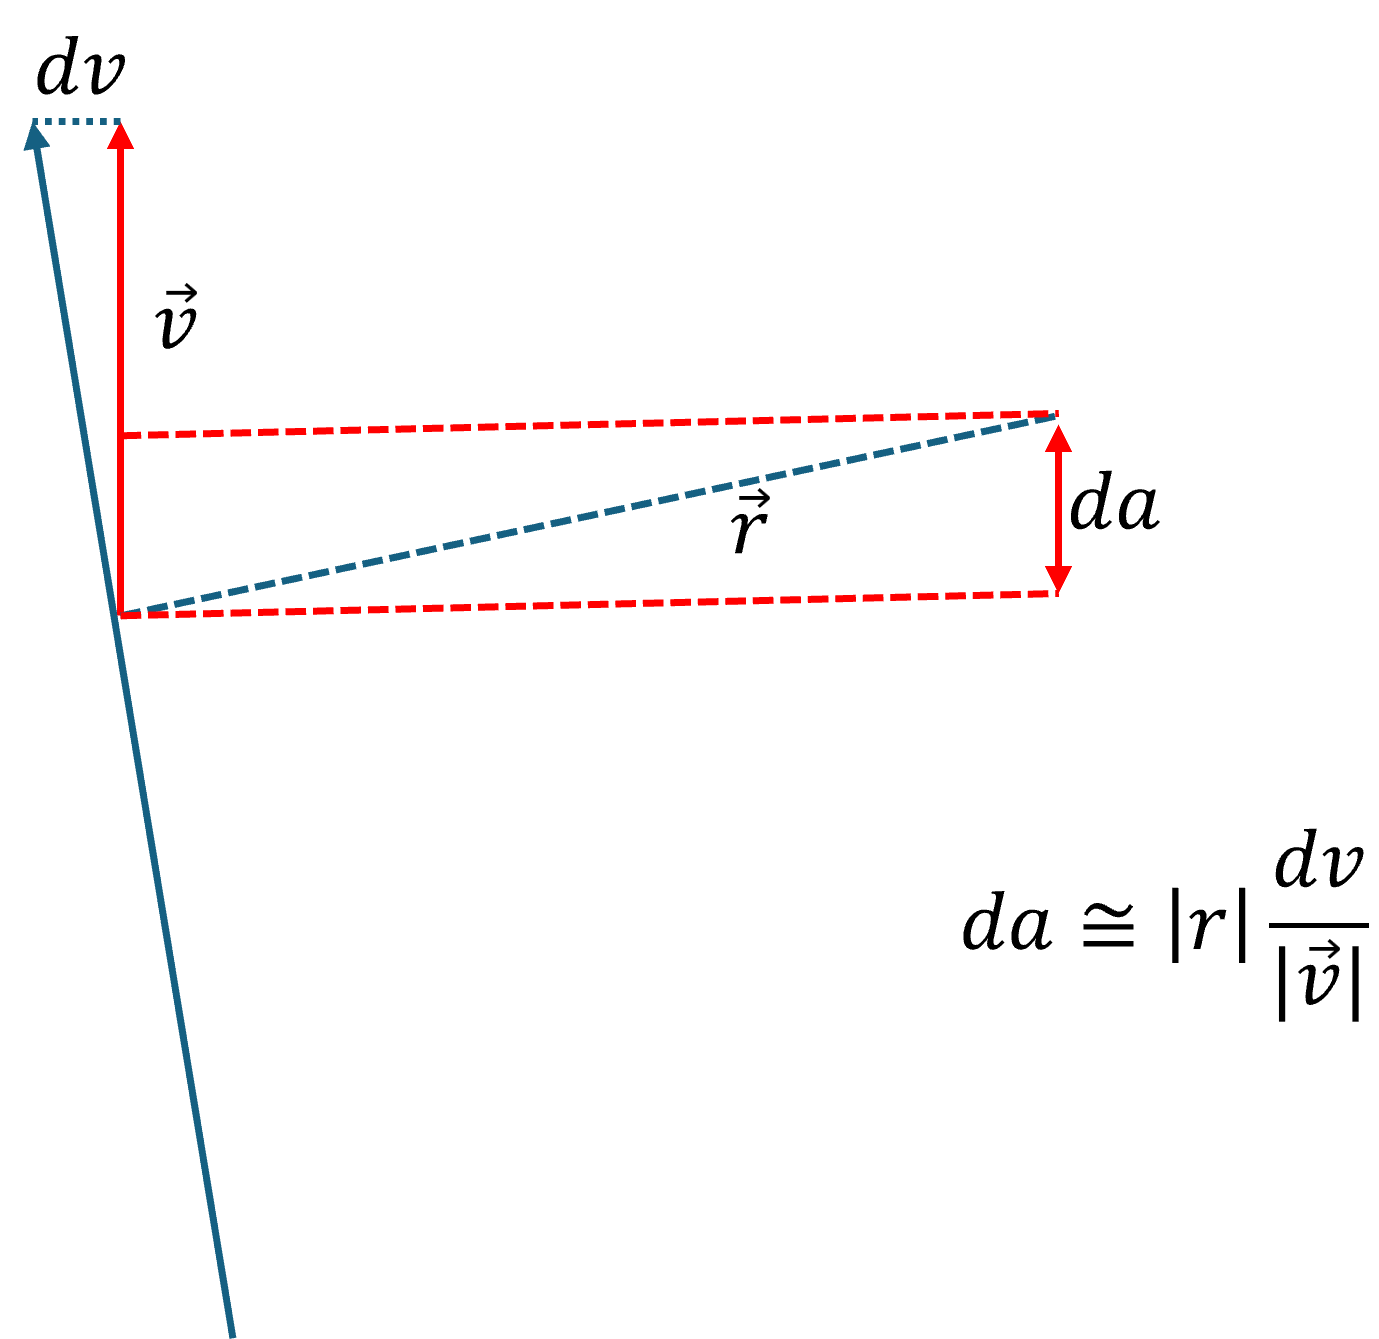
\includegraphics[width=0.4\textwidth]{Figures/cslc/da_graph.png}
\caption{Simple sketch of the acquisition geometry. An error in the velocity direction \(dv\) implies an error in the zero-Doppler determination.}
\label{fig:da_from_dv}
\end{figure}

The standard deviation of the error in azimuth position estimation, denoted $\sigma_{da}$, is given by:

\begin{equation}
\sigma_{da}^2 = \left( \frac{R}{\lVert \mathbf{v} \rVert} \right)^2 \sigma_{v_{\perp}}^2
\label{eq:azimuth_error_baseline}
\end{equation}

where $\lVert \mathbf{v} \rVert$ is the norm of the satellite velocity vector, and $\sigma_{v_{\perp}}$ is the standard deviation in the estimation of its perpendicular component with respect to the line-of-sight. Equation~\ref{eq:azimuth_error_baseline} shows that the azimuth error is directly proportional to $\sigma_{v_{\perp}}$.

This relationship is illustrated in Figure~\ref{fig:azimuth_error_baseline}, which shows the variation of $\sigma_{da}$ as a function of $\sigma_{v_{\perp}}$, assuming constant values of $R = 600000$ m and $\lVert \mathbf{v} \rVert = 7500$ m/s.

\begin{figure}[ht!]
\centering
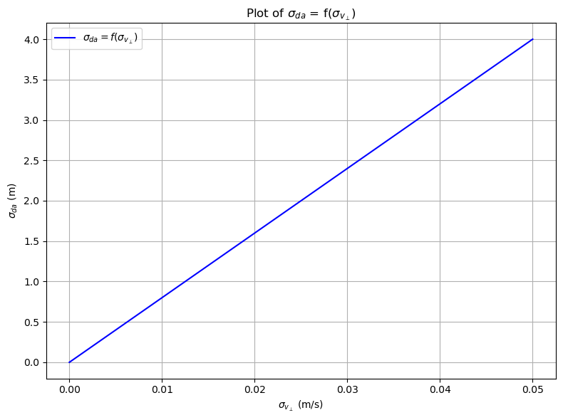
\includegraphics[width=0.9\textwidth]{Figures/cslc/sigma_azimuth.png}
\caption{Standard deviation in azimuth position $\sigma_{da}$ (in meters) as a function of the standard deviation in the perpendicular component of satellite velocity, $\sigma_{v_{\perp}}$, assuming $\lVert \mathbf{v} \rVert = 7500$ m/s and $R = 600000$ m.}
\label{fig:azimuth_error_baseline}
\end{figure}

An error in the input \acs{dem} primarily affects the slant-range positioning, with negligible impact on the azimuth direction. In particular, the standard deviation in slant-range position, $\sigma_{dr}$, previously derived in \ref{eq:slant_range_error_baseline}, must be increased with the following additional term to account for \acs{dem} height uncertainty:

\begin{equation}
\sigma_{dr}^2 = \left( \frac{B_{\perp}}{R \sin\theta} \right)^2 \sigma_{h}^2
\label{eq:eq_slant_range_error_dem}
\end{equation}

Here, $\sigma_{h}$ represents the standard deviation of the elevation error in the input \acs{dem}, and $B_{\perp}$ is the perpendicular component of the baseline between acquisitions. This term is linearly dependent on the height uncertainty, and thus highlights the sensitivity of slant-range accuracy to DEM quality.

Figure~\ref{fig:slant_range_error_dem} illustrates this relationship by showing the resulting $\sigma_{dr}$ values for varying $\sigma_{h}$, assuming $B_{\perp} = 1000$ m, $R = 600000$ m, and $\theta = 40^\circ$.

\begin{figure}[ht!]
\centering
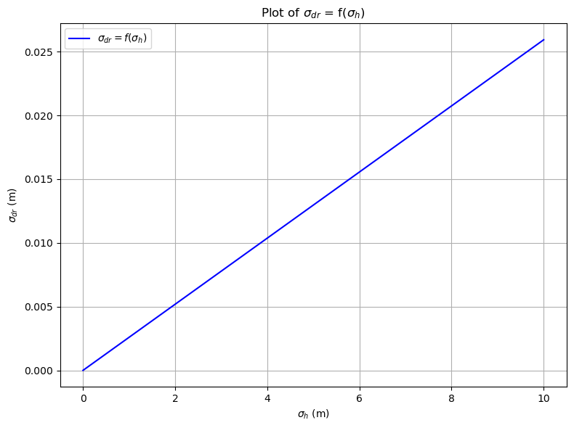
\includegraphics[width=0.9\textwidth]{Figures/cslc/sigma_slant_range_DEM.png}
\caption{Standard deviation in slant-range position $\sigma_{dr}$ (in meters) as a function of the standard deviation in the input \acs{dem} elevation, $\sigma_{h}$, assuming $B_{\perp} = 1000$ m, $R = 600000$ m, and $\theta = 40^\circ$.}
\label{fig:slant_range_error_dem}
\end{figure}

Under nominal conditions, orbital errors on the order of a few centimetres to decimetres and \acs{dem} inaccuracies of a few metres introduce only minor errors in the determination of the slant-range and azimuth positions of ground 3D coordinates. These sources of error can, to a first approximation, be considered negligible—particularly when compared to the significantly larger and more variable errors introduced by atmospheric propagation effects.

Among these, ionospheric and tropospheric delays represent the most prominent contributors. The ionospheric delay is dispersive, and thus strongly dependent on radar frequency. While its impact at C-Band is generally not so relevant (even if it is not completely negligible), it becomes a dominant source of slant range error at L-Band, where uncorrected distortions can exceed several meters—especially in equatorial regions or during periods of geomagnetic disturbance. 

Recent studies have quantified the residual co-registration error achievable with and without atmospheric compensation. Using Sentinel-1 C-band acquisitions over Chile, Zhang \textit{et al.} report an initial slant-range mis-registration \textit{RMSE} of \SI{0.20}{\metre} when only precise orbits and a \acs{dem} are applied; after model-driven corrections for ionosphere, troposphere, and solid-Earth tides, the error decreases to \SI{0.06}{\metre} (0.027 pixels), with 80 \% of scenes below \SI{0.07}{\metre}. In the companion L-band analysis, the uncorrected ALOS-2 stack shows an \textit{RMSE} of \SI{2.66}{\metre}; applying the same suite of atmospheric models reduces the error to \SI{0.56}{\metre}.


\begin{comment}
Our experiments with additional Sentinel-1 tracks (both ascending and descending) confirm the C-band figures: after the identical ionospheric, tropospheric, and tidal corrections, residual range offsets consistently fall in the \SIrange{0.05}{0.07}{\metre} interval—fully consistent with the published \SI{0.06}{\metre} value and well inside the \SI{0.1}{\metre} guideline adopted for ROSE-L quality assurance.  These results reinforce two key conclusions: (i) model-based atmospheric compensation is already sufficient for C-band interferometric applications, and (ii) additional refinement—particularly more accurate, low-latency TEC information—will be essential for meeting the stricter L-band accuracy targets foreseen for ROSE-L.  
HERE WE COULD INSERT THE RESULT IN TERMS OF COREGISTRATION ACCURACY WE HAVE USING AND NOT USING THE ETAD CASE SENTINEL-1
\end{comment}

Although the cited study maintains that the proposed model is sufficient to support image co-registration in interferometric applications, its direct extension to ROSE-L is not straightforward due to several key limitations:

\begin{itemize}
    \item The analysis does not consider azimuthal ionospheric effects, which can be as significant as range offsets in precise co-registration scenarios.
    
    \item The results are based on ALOS-2 acquisitions around 12:00 local solar time, a period typically associated with relatively mild ionospheric conditions. In contrast, \acs{rosel} is expected to acquire data near 18:00 local solar time, when ionospheric disturbances—particularly  at high latitudes (e.g., near the polar regions) or during periods of elevated solar activity—tend to be more severe. By extrapolating from ascending Sentinel-1 data (acquired at 18:00) and adjusting for the L-band wavelength scaling factor, an expected 1-sigma slant-range offset of approximately 1.6~m can be derived ($8.7~\text{cm} \times (\lambda_L/\lambda_C)^2$), which approaches the nominal slant-range resolution of \acs{rosel} (2.5~m). This level of error is too large to meet interferometric performance requirements.
    
    \item The study assumes a system bandwidth of 24~MHz, as used in the \acs{nisar} scenario. However, for \acs{rosel}'s standard mode (RIWS), the effective bandwidth may reach up to 60~MHz. This increases the sensitivity to range errors, thereby making \acs{rosel}’s ionospheric requirements significantly more stringent.
    
    \item Finally, the ionospheric correction performance in the referenced study relies on the use of JPL’s high-resolution ionosphere model (“JHR”), which is neither publicly available nor guaranteed in terms of latency or accessibility for operational processing pipelines.
\end{itemize}

All of these considerations must be carefully accounted for in the definition of co-registration and geolocation accuracy requirements. In particular, the requirements should be specified with respect to worst-case scenarios—such as acquisitions at high latitudes (e.g., polar regions) or during periods of elevated solar activity—where ionospheric disturbances are typically more severe. It is equally important to acknowledge that under more favorable conditions, such as acquisitions over equatorial or mid-latitude regions during geomagnetically quiet periods, significantly improved performance can be expected. In such cases, the achievable accuracy may exceed the baseline requirements by up to an order of magnitude.


To verify that the theoretical error budget presented here is achievable in practice, we performed a dedicated co-registration experiment using a Sentinel-1 image stack acquired over the Surat Basin, Australia, where a network of calibrated corner reflectors (CRs) is permanently installed.  All CRs with radar-cross-section \(>\) 35 dBsm were retained as control targets. Two sets of \acs{cslc}s were generated with respect to a single master \acs{slc}:  
\begin{itemize}
    \item using only precise orbits and the 30 m SRTM DEM;   
    \item unsing also the \acs{etad} layers were additionally applied to compensate tropospheric and ionospheric delays.
\end{itemize}

For every slave image and for each visible CR, the residual offset vector \(\Delta r\) (slant range) and \(\Delta a\) (azimuth) was measured as the sub-pixel displacement between the CR’s peak position in the master and in the resampled slave.  Sub-pixel locations were estimated by oversampling (with a sinc interpolator) both master and co-registered slave in corrispondence on the CR response.

Figure~\ref{fig:delta_coreg_before_etad} shows the accuracy achieved using only orbital and DEM information, while Figure~\ref{fig:delta_coreg_after_etad} presents the results obtained when \acs{etad} corrections are included in the co-registration process.

In both figures, the $x$-axis lists the identifiers of the corner reflectors (CRs) used in the analysis, and the $y$-axis reports the measured mis-registration in slant range (left) and azimuth (right), both expressed in metres.
Each dot represents the residual offset for a single CR; different colours correspond to different slave images co-registered to the same master.

By comparing the two plots, it becomes evident that atmospheric delays—although modest at C-band—introduce a systematic error in slant range when not corrected.
In Figure~\ref{fig:delta_coreg_before_etad}, each slave shows a distinct mean offset in range, visible as a vertical shift across CRs of the same colour. This is consistent with the slow spatial variability of tropospheric and ionospheric delays, which act primarily as a constant bias in slant range.
The azimuth direction is less affected, showing minimal variation in both mean and spread.

When \acs{etad} information is used (Figure~\ref{fig:delta_coreg_after_etad}), this systematic range bias is significantly reduced, aligning the mean residuals closer to zero.
While the standard deviation (i.e., the random component) remains nearly unchanged, the correction of the constant bias enhances absolute co-registration accuracy.
This confirms that—even at C-band—accounting for atmospheric delays improves product consistency, particularly in applications requiring high geometric precision.

\begin{figure}[ht!]
\centering
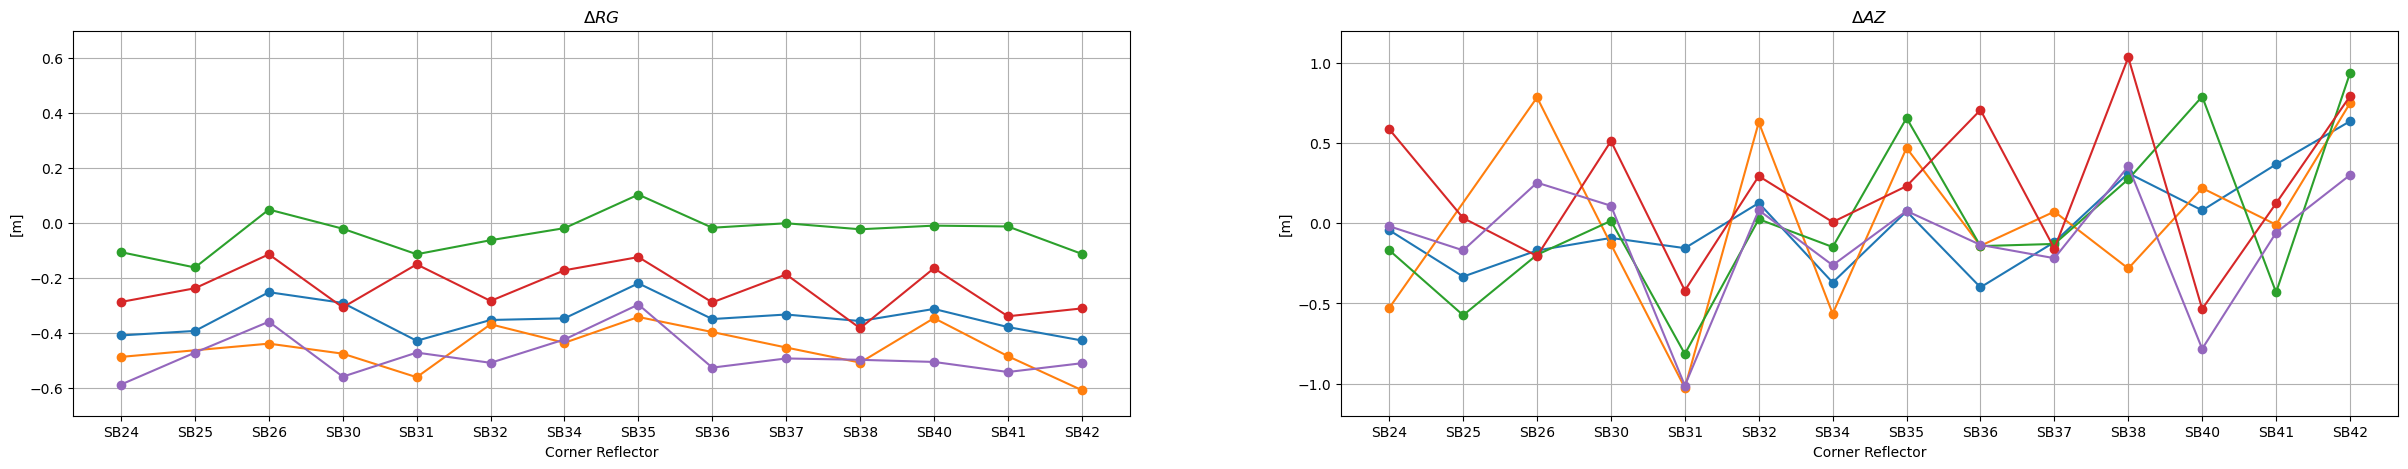
\includegraphics[width=0.9\textwidth]{Figures/cslc/delta_coreg_before_etad.png}
\caption{Co-registration errors using only orbital and DEM information. Each dot shows the mis-registration (in metres) of a corner reflector in slant range (left) and azimuth (right). Colours indicate different slave images.}
\label{fig:delta_coreg_before_etad}
\end{figure}


\begin{figure}[ht!]
\centering
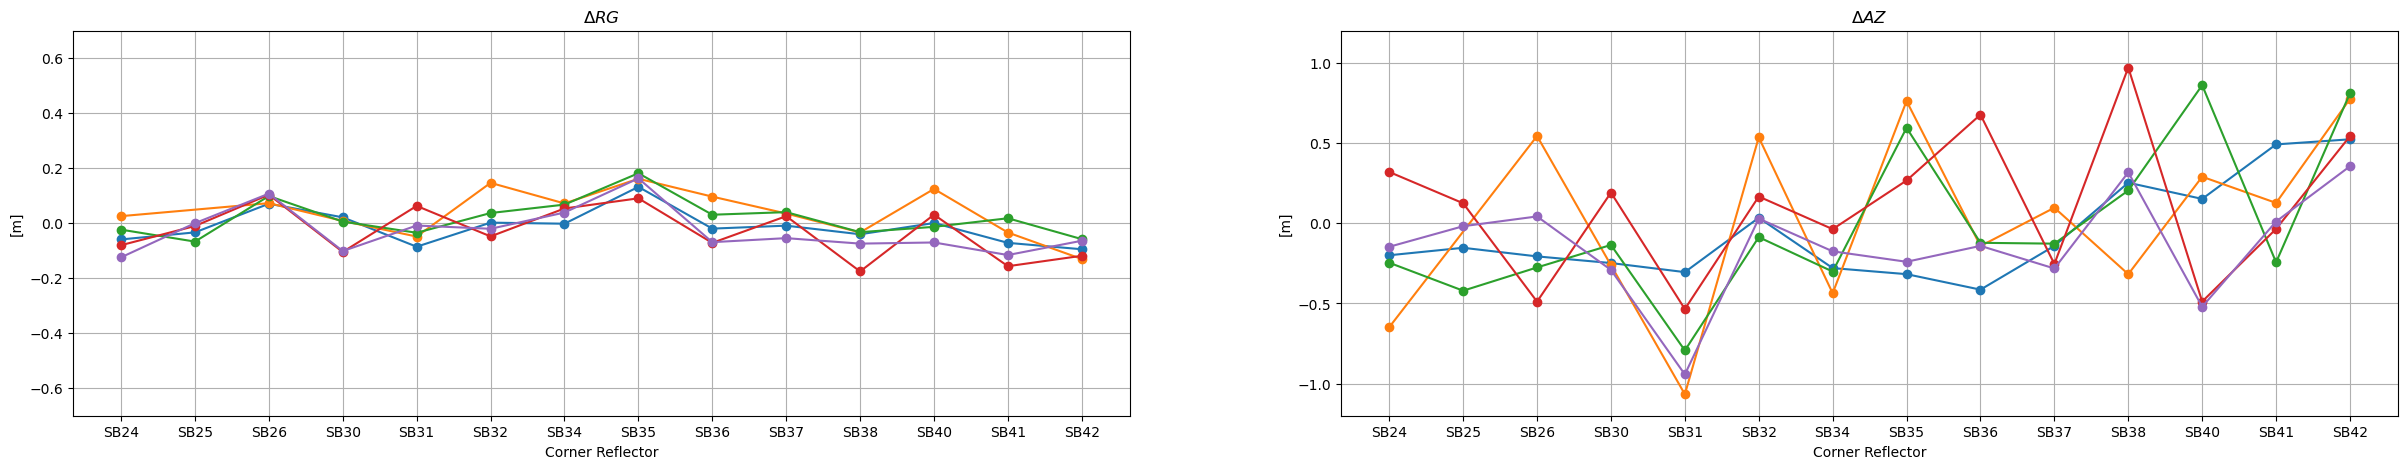
\includegraphics[width=0.9\textwidth]{Figures/cslc/delta_coreg_after_etad.png}
\caption{Co-registration errors using orbital, DEM, and ETAD information. The systematic range bias visible in Figure~\ref{fig:delta_coreg_before_etad} is largely corrected. The azimuth alignment remains stable in both cases.}
\label{fig:delta_coreg_after_etad}
\end{figure}
In the Co-registration, the following parameters have been used:
\begin{itemize}
    \item warp\_ov\_fact, number of samples used to generate the sinc function: 100000
    \item warp\_kernel\_shape, shape of the interpolation kernel (height, width): [11,11]
    \item warp\_kaiser\_beta, beta parameter for the Kaiser window used to weight the sinc function: 6
\end{itemize}

\subsubsection{Absolute geolocation accuracy}
\label{sec:gslc_absolute_geolocation_accuracy}

In order to evaluate the absolute geolocation accuracy of the projected product (\acs{gslc}), the following elements must be considered: the vertical and horizontal accuracy of the \acs{dem}, and the accuracy in determining the range and azimuth coordinates in the \acs{slc} images. The relationship linking geolocation accuracy with input data accuracy, in the zero-Doppler plane, can be explained starting from the acquisition geometry sketch shown in Figure~\ref{fig:gslc_geolocation_accuracy}.

\begin{figure}[ht!]
\centering
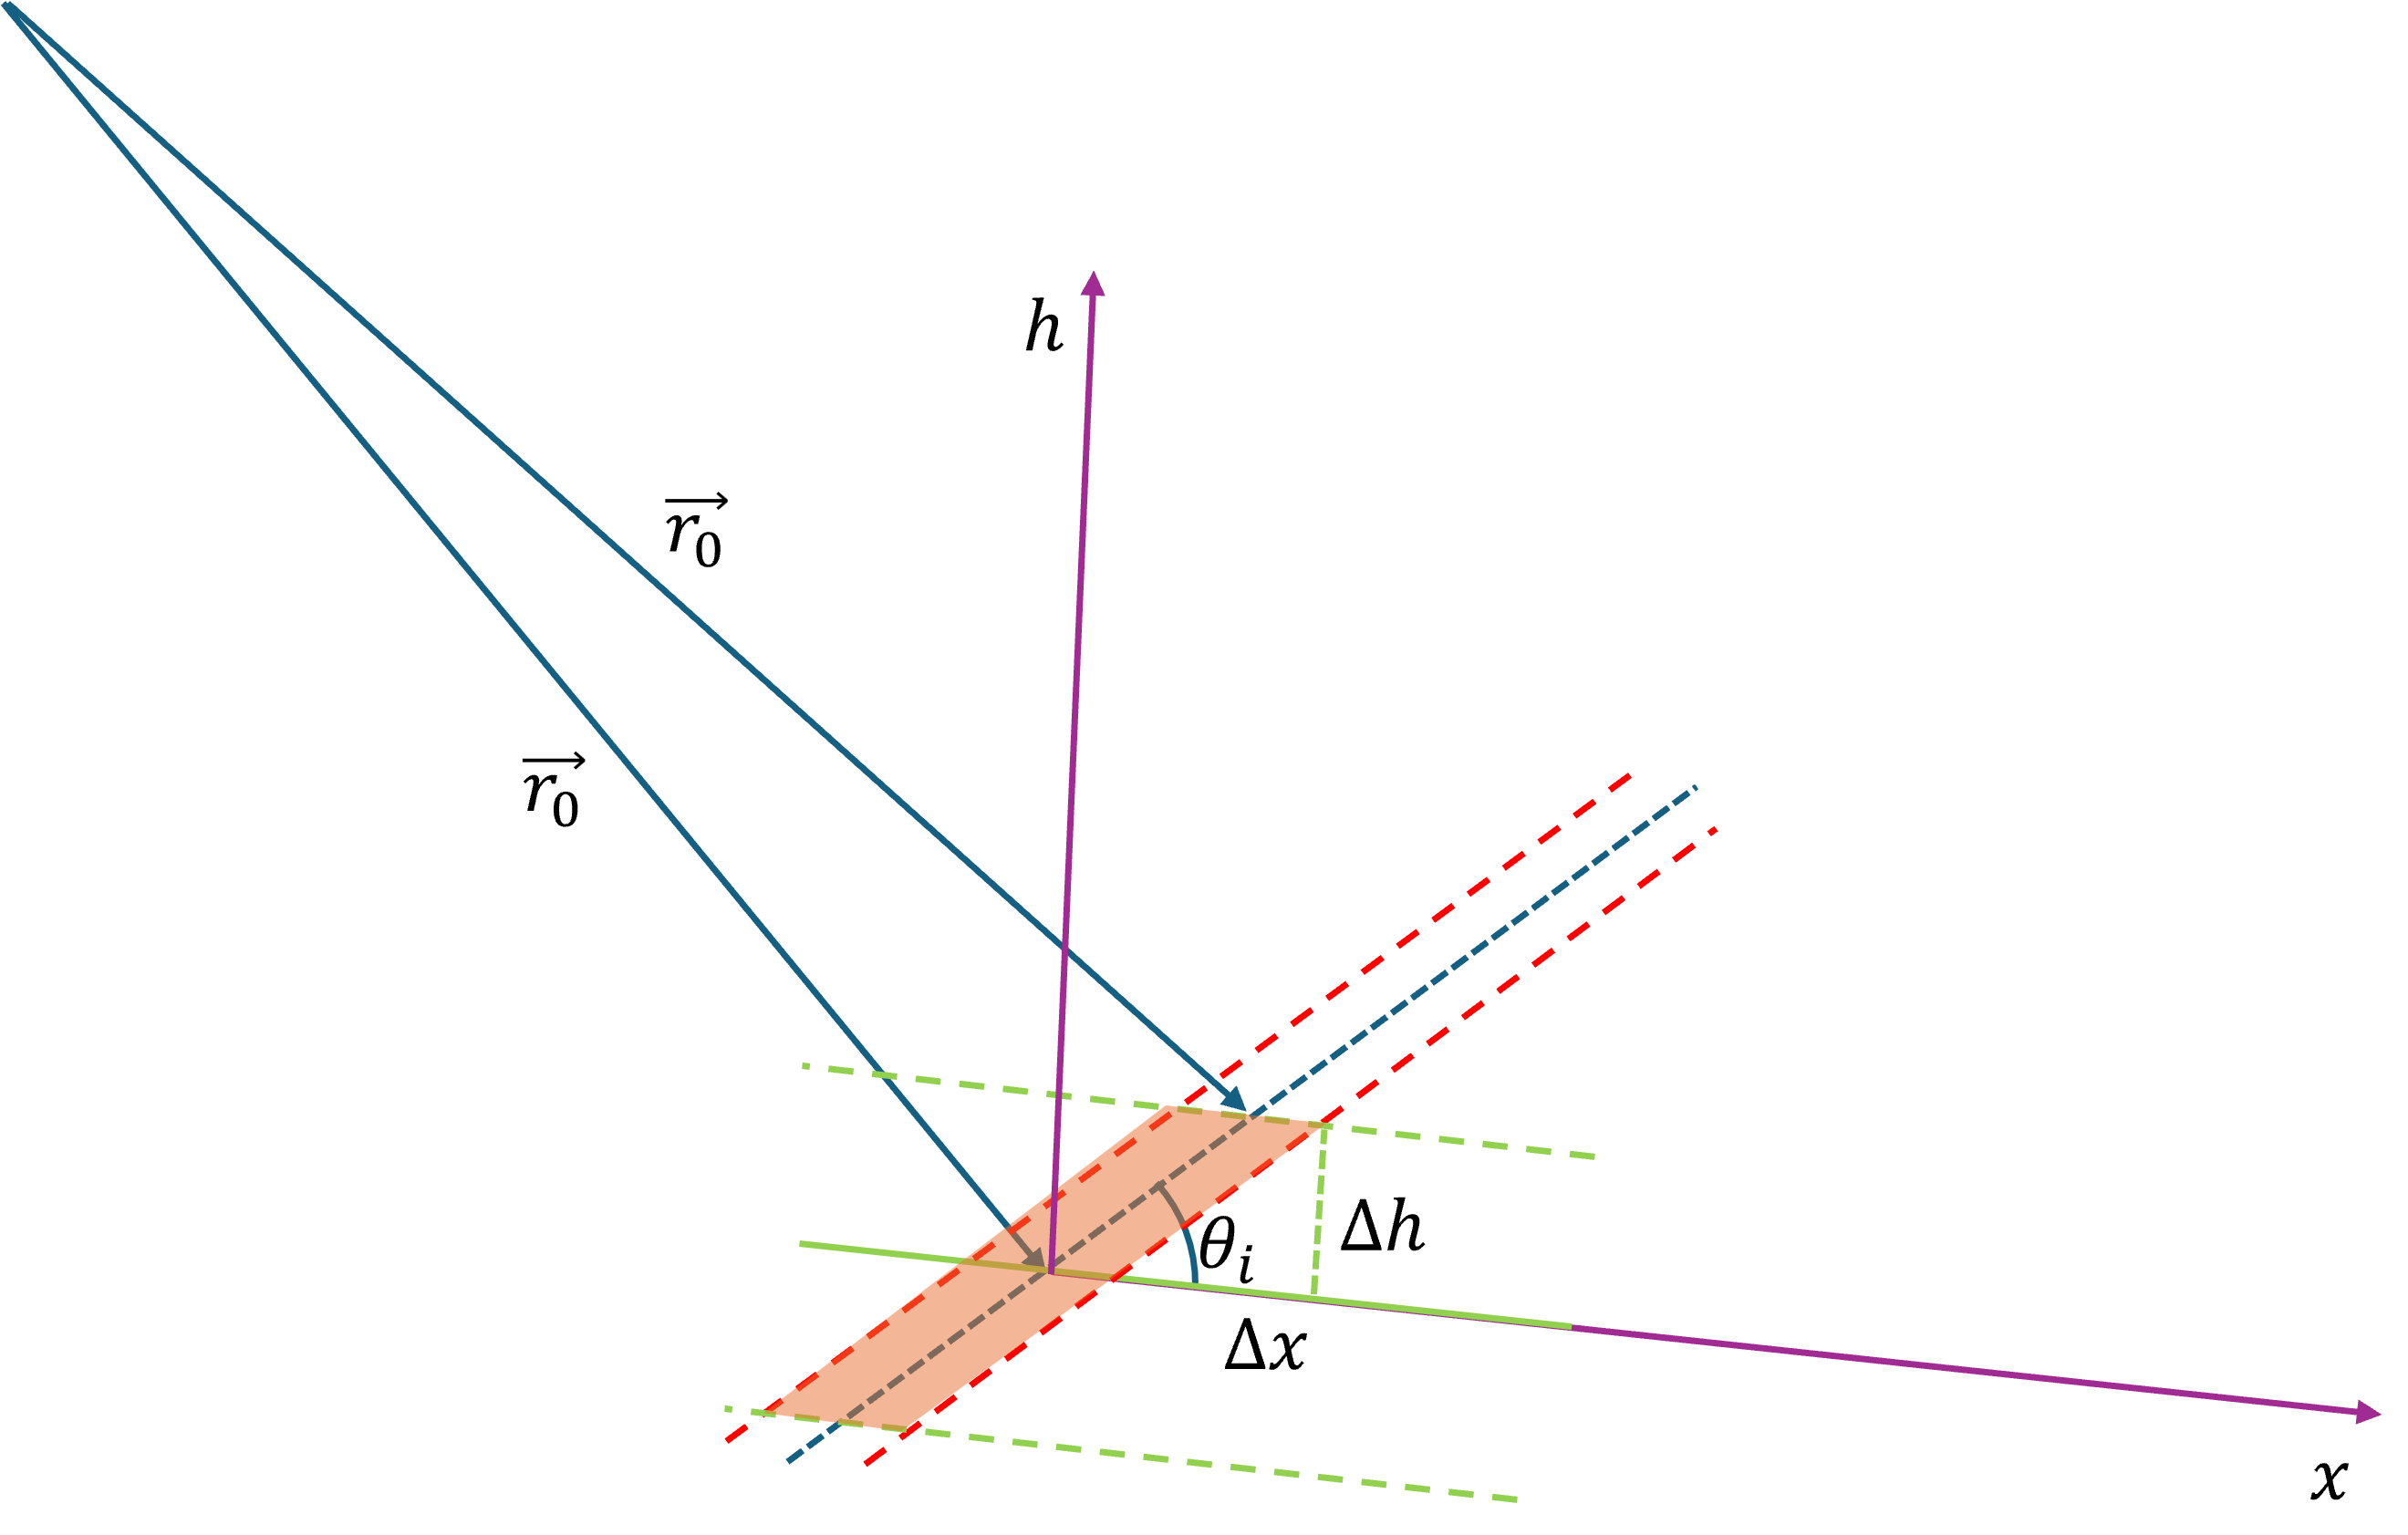
\includegraphics[width=0.9\textwidth]{Figures/cslc/geolocation_accuracy.png}
\caption{Simplified sketch of the acquisition geometry of a single SAR image in the zero-Doppler plane. The localization error of a ground point results from the combined uncertainty in the slant-range position and the \acs{dem} surface.}
\label{fig:gslc_geolocation_accuracy}
\end{figure}

The area where the point can be geolocated is constrained by the error in slant-range position (red dashed lines) and the error in elevation (green dashed lines).  
Let $\alpha$ be the local slope, $\theta_i$ the local incidence angle, $\sigma^{DEM}_x$ and $\sigma^{DEM}_h$ the horizontal and vertical accuracy of the input \acs{dem}, and $\sigma_{dr}$ the slant-range accuracy of the input \acs{slc}. The final error in the $x$ coordinate is given by:

\begin{equation}
\sigma_{dx}^2 = \frac{\sigma^2_h}{\tan^2 \theta_i} + \frac{\sigma^2_{dr}}{\sin^2 \theta_i} = \frac{\left(\sigma^{DEM^2}_x \tan^2 \alpha + \sigma^{DEM^2}_h\right)}{\tan^2 \theta_i} + \frac{\sigma^2_{dr}}{\sin^2 \theta_i}
\label{eq:gslc_dx_accuracy}
\end{equation}

When ETAD corrections are applied, the error in slant-range position is reduced to a few centimeters, both in terms of bias and standard deviation. Therefore, the second term (slant-range) in Equation~\ref{eq:gslc_dx_accuracy} becomes negligible compared to the first term (\acs{dem}), which is typically one order of magnitude larger. Without ETAD corrections, both sources of error are comparable and typically on the order of few meters.

\subsubsection{Radiometric quality}
\label{sec:cslc_radiometric_quality}

The evaluation of radiometric fidelity for the \acs{cslc} product is theoretically grounded in the analysis of key image quality indicators, namely Spatial Resolution, Peak Side-Lobe Ratio (\acs{pslr}), and Integrated Side-Lobe Ratio (\acs{islr}). These metrics are derived from the impulse response of point scatterers and provide insight into the integrity of the SAR signal following resampling.

In the generation of \acs{cslc} products, co-registration is achieved by interpolating the slave image to the master’s geometry. This process uses a finite-length sinc interpolator modulated by a Kaiser window. The sinc kernel, by design, preserves the frequency content of the original signal, ensuring minimal degradation in spatial resolution. The Kaiser window serves to suppress the side lobes of the interpolator's response, thereby mitigating increases in \acs{pslr} and \acs{islr}.

Theoretically, such an interpolation strategy is expected to introduce very limited radiometric degradation. Provided the interpolation kernel is sufficiently long and well-parameterized, the resulting \acs{cslc} product should retain the spatial and radiometric quality of the input \acs{slc} data with negligible impact.

This expectation is supported by standard SAR signal processing literature, which demonstrates that sinc interpolation with appropriate windowing results in minimal loss of resolution and side-lobe performance \cite{Cumming2005}, \cite{Moreira2013}, \cite{Soumekh1999}. Accordingly, any deviations observed in practice are more likely attributable to implementation or data-specific effects rather than inherent limitations of the resampling approach. 

To assess the impact of the co-registration process on radiometric quality, the differences in Integrated Side-Lobe Ratio (\acs{islr}) and Peak Side-Lobe Ratio (\acs{pslr}) between co-registered \acs{slc} products (\acs{cslc}) and their original \acs{slc} counterparts were computed. These differences are visualized in Figures~\ref{fig:PSLR_comparison} and~\ref{fig:ISLR_comparison}, using a comprehensive set of Corner Reflectors (\acs{cr}s) with Radar Cross Sections exceeding 35 dBsm. 

For each CR and for each image pair (original and co-registered), \acs{islr} and \acs{pslr} were estimated independently in both the slant-range and azimuth directions. The x-axis of each plot shows the original metric value as measured on the \acs{slc}, while the y-axis shows the corresponding difference observed after co-registration. 

Each dot represents an individual CR; dots sharing the same color refer to CRs measured within the same image. Color changes denote a change in the input \acs{slc} scene. This visualization enables the detection of systematic biases or degradations introduced by the co-registration step and confirms the expected minimal impact on radiometric sharpness indicators.

\begin{figure}[h!]
\centering
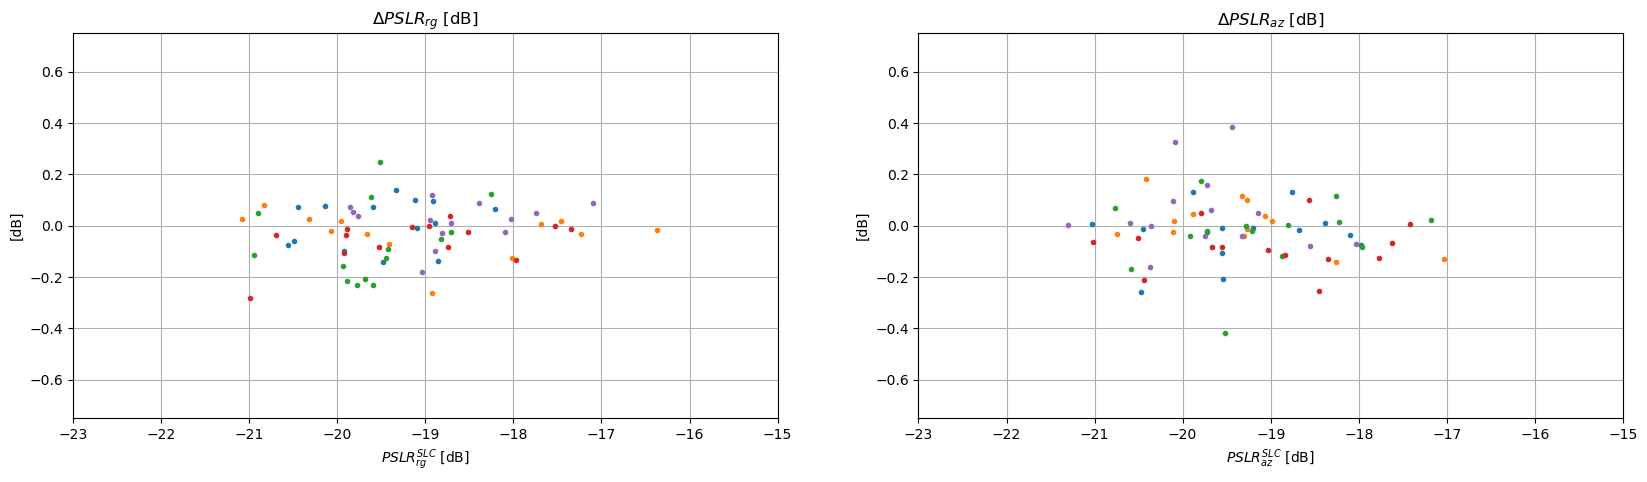
\includegraphics[width=0.9\textwidth]{Figures/cslc/PSLR_comparison.png}
\caption{Difference in Peak Side-Lobe Ratio (\acs{pslr}), expressed in dB, between co-registered \acs{slc} products (\acs{cslc}) and their original \acs{slc} counterparts. The left panel shows the \acs{pslr} difference in slant-range direction, while the right panel shows the difference in azimuth. The x-axis represents the original \acs{pslr} value (in dB) as measured on the \acs{slc}, and the y-axis shows the difference $\text{PSLR}^{\text{CSLC}} - \text{PSLR}^{\text{SLC}}$. Each dot corresponds to a single Corner Reflector (\acs{cr}) with Radar Cross Section (\acs{rcs}) greater than 35 dBsm. Dots of the same color refer to \acs{cr}s within the same image; changes in color indicate different \acs{slc}.}
\label{fig:PSLR_comparison}
\end{figure}

\begin{figure}[h!]
\centering
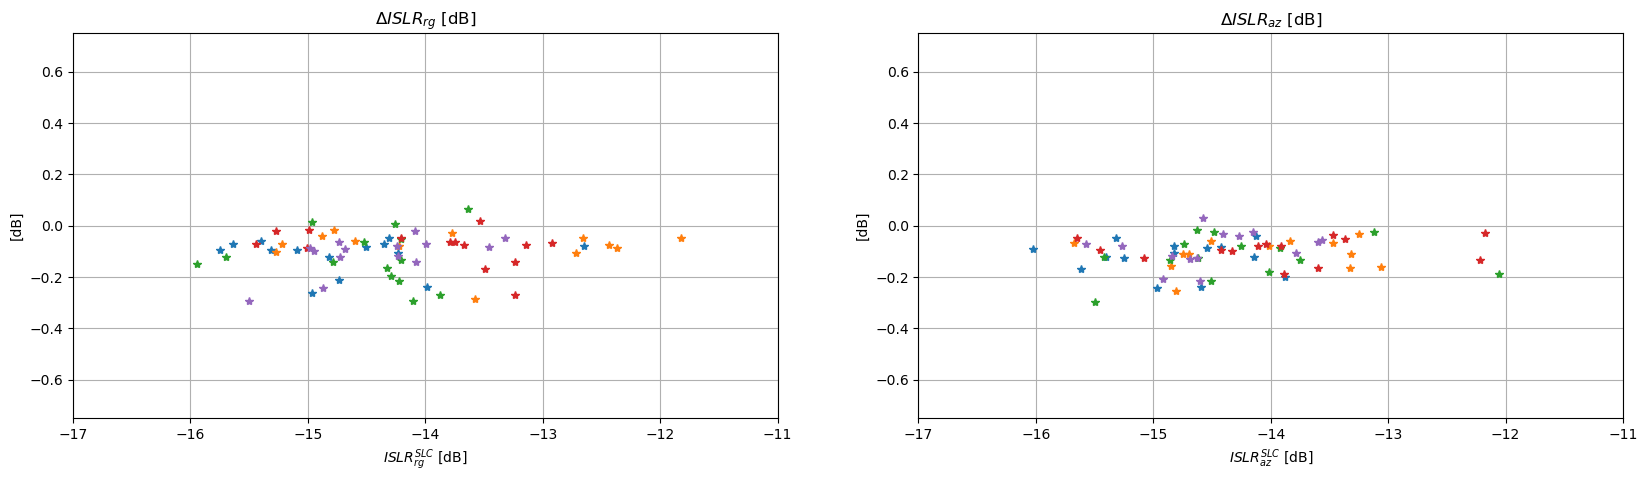
\includegraphics[width=0.9\textwidth]{Figures/cslc/ISLR_comparison.png}
\caption{Difference in Integrated Side-Lobe Ratio (\acs{islr}), expressed in dB, between co-registered \acs{slc} products (\acs{cslc}) and their original \acs{slc} counterparts. The left panel shows the \acs{islr} difference in slant-range direction, while the right panel shows the difference in azimuth. The x-axis represents the original \acs{islr} value (in dB) as measured on the \acs{slc}, and the y-axis shows the difference $\text{ISLR}^{\text{CSLC}} - \text{ISLR}^{\text{SLC}}$. Each dot corresponds to a single Corner Reflector (\acs{cr}) with Radar Cross Section (\acs{rcs}) greater than 35 dBsm. Dots of the same color refer to \acs{cr}s within the same image; changes in color indicate different \acs{slc}.}
\label{fig:ISLR_comparison}
\end{figure}

In addition to \acs{islr} and \acs{pslr}, the potential impact of co-registration on spatial resolution was assessed. Figure~\ref{fig:spatial_resolution_comparison} presents the resolution difference, expressed in meters, between the co-registered \acs{slc} (\acs{cslc}) and the original \acs{slc}, evaluated separately in slant-range (left panel) and azimuth (right panel) directions.

The x-axis in each panel reports the spatial resolution measured on the original \acs{slc} product, while the y-axis shows the corresponding resolution difference after co-registration. As with the previous figures, each point corresponds to a single \acs{cr} (\acs{rcs} > 35 dBsm), and colors are used to distinguish \acs{cr}s across different \acs{slc} scenes.

The plots confirm that spatial resolution remains stable across all analyzed scenes and directions, further supporting the conclusion that the applied co-registration method introduces negligible degradation in radiometric sharpness and point target response.

\begin{figure}[h!]
\centering
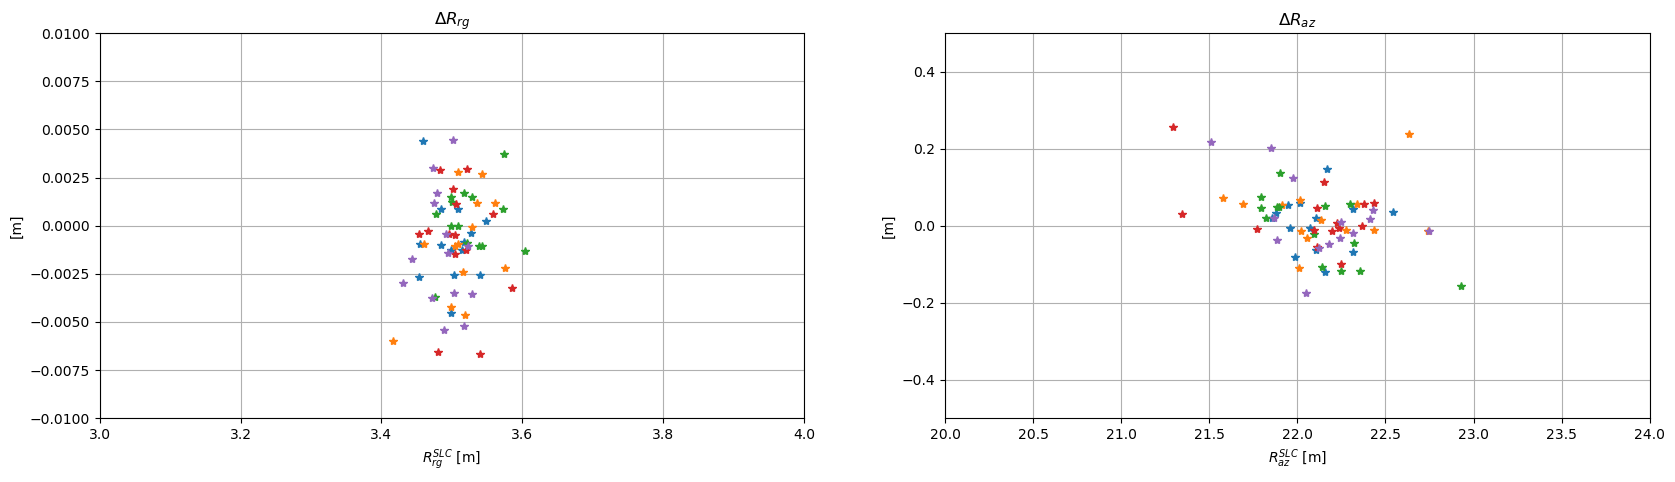
\includegraphics[width=0.9\textwidth]{Figures/cslc/spatial_resolution_comparison.png}
\caption{Difference in spatial resolution (in metres) between the co-registered \acs{slc} product (\acs{cslc}) and the original \acs{slc}. The left panel shows the difference in slant-range resolution, and the right panel in azimuth resolution. The x-axes report the original spatial resolution of the \acs{slc} product in each direction. Each point corresponds to a Corner Reflector with \acs{rcs} greater than 35 dBsm. As in previous figures, dots of the same color indicate \acs{cr}s extracted from the same image, while color changes correspond to different input \acs{slc} scenes.}
\label{fig:spatial_resolution_comparison}
\end{figure}

\begin{figure}[h!]
\centering
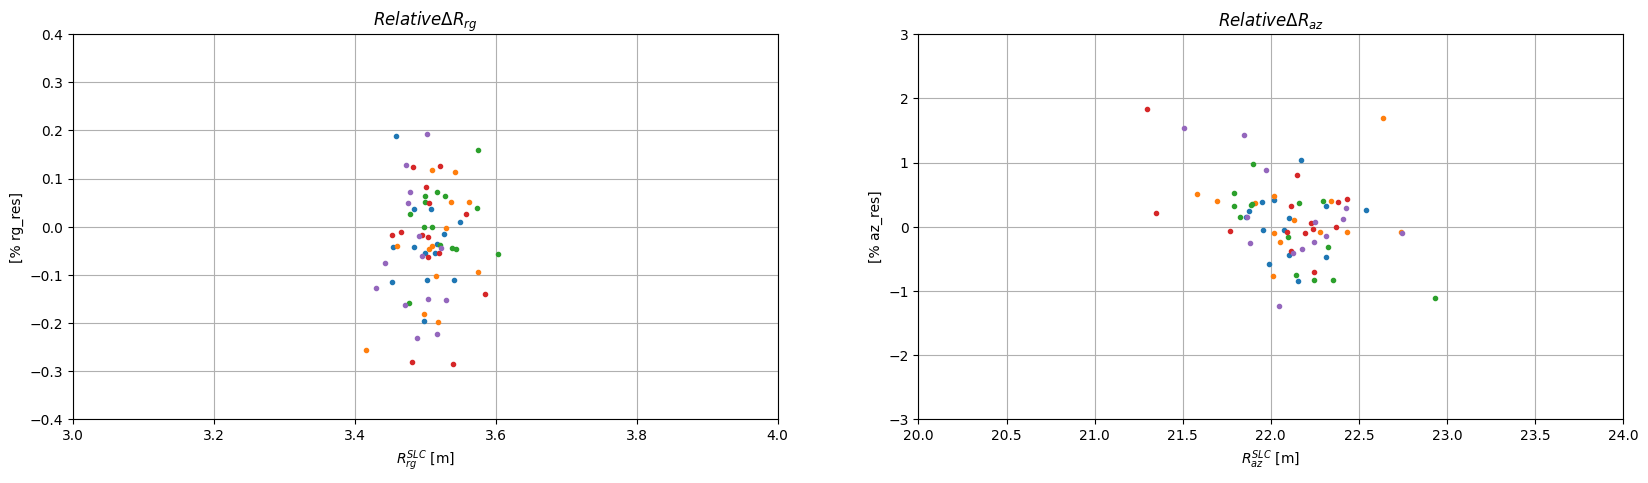
\includegraphics[width=0.9\textwidth]{Figures/cslc/spatial_resolution_comparison_relative.png}
\caption{Relative difference in spatial resolution (percentage with respect to the satellite resolution) between the co-registered \acs{slc} product (\acs{cslc}) and the original \acs{slc}. The left panel shows the difference in slant-range resolution, and the right panel in azimuth resolution. The x-axes report the original spatial resolution of the \acs{slc} product in each direction. Each point corresponds to a Corner Reflector with \acs{rcs} greater than 35 dBsm. As in previous figures, dots of the same color indicate \acs{cr}s extracted from the same image, while color changes correspond to different input \acs{slc} scenes.}
\label{fig:spatial_resolution_comparison_relative}
\end{figure}


The theoretical framework for evaluating the radiometric fidelity of the \acs{gslc} product follows similar principles to those applied for the \acs{cslc}. In particular, the geocoding process employs a finite-length sinc interpolator modulated by a Kaiser window, which is theoretically well-suited to preserving signal integrity. This approach ensures minimal degradation of the original \acs{sar} signal, particularly when the ground sampling interval is chosen to match the nominal resolution of the sensor as closely as possible.

However, unlike the \acs{cslc}, the transformation from radar to ground coordinates introduces additional challenges that could affect the radiometric quality indicators. In particular:

\begin{itemize}
    \item \textbf{Topographic distortion effects}: Elevation variation causes geometric distortions such as foreshortening, layover, and shadowing in the geocoded image, which can degrade the shape and sharpness of point target responses.
    \item \textbf{Geolocation-induced rotation}: The projection from radar to geographic coordinates results in a rotation of the image grid, misaligning the slant-range and azimuth directions with the map axes. This can distort the impulse response function, making resolution and side-lobe measurements less consistent.
    \item \textbf{\acs{dem} dependency}: The accuracy of the geocoding process depends heavily on the quality of \acs{dem}. Errors in the \acs{dem} can lead to geometric misregistration, signal smearing, and local inaccuracies.
\end{itemize}

As a consequence, while the theoretical interpolation scheme remains robust, these secondary effects can lead to measurable degradation in image quality indicators such as Spatial Resolution, \acs{islr}, and \acs{pslr}. Furthermore, the geometric transformations applied during geocoding make it more complicated to obtain a reliable estimate of these indicators.

Therefore, these considerations should be reflected in the product specifications used to assess whether the geocoding process has been implemented correctly and within acceptable tolerances. 



\subsection{Computational performance}
\label{sec:cslc_computation}

\subsubsection{Co-registration Workflow}

The computational load of co-registering a slave image to a master grid is dominated by three successive operations.

\paragraph{\acs{dem} to radar coordinate conversion}  
Processing begins by mapping every node of the Digital Elevation Model (\acs{dem}) covering the Area Of Interest (AOI) into radar coordinates.  
For each \acs{dem} triplet $(x,y,z)$ the algorithm solves the range–Doppler equations to obtain the slant-range distance $r$ and the zero-Doppler azimuth time $t$.  
Because the system is non-linear, an iterative Newton–Raphson search is required, typically converging in five to eight iterations.  
Hence the cost grows linearly with the number of \acs{dem} nodes, $K\!\propto\!\text{AOI}/\Delta_{\text{DEM}}^{2}$.  
For example, a 100 km × 100 km scene sampled at 30 m already involves $\sim$11 million DEM points.

\paragraph{Interpolation of the sparse control mesh}  
The resulting tie points $\{(r_i,t_i)\}$ form an irregular control mesh that must be interpolated onto the master’s regular radar grid.  
A common strategy is to build a Delaunay triangulation (cost $\mathcal{O}(K\log K)$) and then apply barycentric interpolation; each master pixel is evaluated in constant time with three multiplications and two additions.


\paragraph{Image warping with a sinc–Kaiser kernel}  
Finally, the slave signal is resampled onto the master grid.  
For every output pixel the algorithm evaluates a finite two-dimensional sinc kernel apodised by a Kaiser window.  
With an \(M\times N\) kernel the operation count is \(MN\) multiplications plus \(MN-1\) additions per pixel; high-fidelity implementations typically use a kernel of at least \(11\times11\).

\bigskip
\noindent
In summary, the DEM projection cost scales with AOI size and DEM spacing, while the warping stage scales with the number of output pixels and the chosen kernel width.  Exploiting multi-core CPUs or GPUs is therefore essential for wide-swath, high-resolution production environments.

\paragraph{Optional cross–correlation refinement}  
When orbit and \acs{dem} information alone are insufficient to guarantee sub-pixel alignment (and there are not any other auxiliary data to be used to improve the co-registration accuracy), an image-based refinement is applied on a sparse grid of control patches. This refinement can use either frequency-domain spectral diversity or spatial cross-correlation. For the latter, small window pairs (e.g.\ $64\times64$ pixels) are extracted at regular spacing and matched to estimate residual offsets.

Implementing cross-correlation requires an additional processing loop:  
\begin{itemize}
\item a coarse-warp of the slave image based solely on geometric information;  
\item cross-correlation of the coarse-warped slave against the master to update the correspondence map; and  
\item a fine-warp using the refined offsets.  
\end{itemize}
This strategy effectively doubles the computational cost of the sinc–Kaiser warp, yet it is often indispensable for achieving the sub-pixel co-registration accuracy demanded by high-coherence interferometry.

\subsubsection{Geocoding Workflow}

Geocoding—the mapping of radar samples onto a ground-projected grid—shares two of the three co-registration steps.

\paragraph{Ground-grid definition and DEM projection}  
A regular ground lattice \((X,Y)\) (e.g.\ UTM or UPS) is first defined at the desired posting, typically chosen close to the native radar resolution.  The height of each ground node, \(h(X,Y)\), is obtained by bilinear or bicubic interpolation of the \acs{dem}.  Each 3-D point \((X,Y,h)\) is then projected into radar coordinates via the same range–Doppler inversion used in co-registration.  Consequently, the computational burden of this stage mirrors the \acs{dem} to radar conversion discussed earlier, with the additional cost of \acs{dem} interpolation.

\paragraph{Direct resampling of the radar image}  
Because every ground node already carries its radar coordinates, no intermediate triangulation is required.  The SAR amplitude or complex value is extracted directly by sinc–Kaiser interpolation at the fractional \((r,t)\) location, and the result is written to the output pixel.  The arithmetic per pixel is identical to the warp step in co-registration; hence the total cost scales linearly with the number of ground-grid cells.

\paragraph{Practical considerations}  
Geocoding performance is highly sensitive to the chosen ground posting. For example, switching from a 40 m grid to a 20 m grid multiplies the number of output pixels (and thus the runtime and I/O) by a factor of four.  Selecting the coarsest spacing that still satisfies application requirements can therefore reduce processing load by an order of magnitude.

\vspace{0.5em}

\noindent
In operational production systems the co-registration and geocoding workflows are executed on the same high-performance nodes: the \acs{dem} projection is performed once and reused by both tasks, followed by either the slave-to-master warp (co-registration) or the direct ground resampling (geocoding).  This strategy maximizes cache reuse, minimizes repeated DEM access, and yields balanced throughput for large-scale \acs{ard} production.

\noindent%
A number of additional processing blocks—such as ingesting timing and solid-Earth-tide \acs{etad} correction layers, and evaluating external ionospheric models—are also executed within the co-registration and geocoding chains; however, these tasks involve only per-pixel table look-ups or simple arithmetic and are computationally negligible compared with the DEM projection, mesh interpolation, and sinc–Kaiser resampling steps detailed above.

\subsection{Criticalities and weakness}
\label{sec:cslc_criticalities}

\subsubsection{Sentinel-1 (C-band)}  
For C-band data, tropospheric and ionospheric delays are modest but not negligible.  
Achieving the highest co-registration accuracy therefore benefits from ingesting \acs{etad} timing layers, which model both tropospheric path delay and ionospheric group delay.  
Precise \acs{etad} products are typically released a few days after acquisition (rapid set: \(\sim\)5 days; final set: \(\sim\)20 days), so their use inevitably reduces product timeliness.  
Nevertheless, theoretical error budgets and extensive empirical tests show that—even without \acs{etad}—the residual mis-registration remains below the threshold required for conventional interferometric applications (e.g.\ interferogram and coherence generation, DInSAR time-series).  
In practice, a geometry-only \acs{cslc} stack built from Sentinel-1 data based on a virtual reference image (no real reference is needed), satisfies most operational needs.

\subsubsection{\acs{rosel} (L-band)}
\label{sec:cslc_criticalities_rosel}

For L-band, atmospheric delays are an order of magnitude larger and cannot be ignored.  
Using geometry alone—or even geometry supplemented with external models such as \acs{etad} or alternatively the JPL high-resolution TEC map, even if the last one is not publicly available—does not reliably meet the stringent accuracy required for interferometric coherence.  
Consequently, ROSE-L co-registration must employ a real \acs{slc} master (a virtual master is inadequate) and refine the geometry with both image-based cross-correlation and spectral-diversity measurements.  
This requirement introduces two operational elements to be considered:
\begin{itemize}
\item \textbf{Reference-image selection}. The master should exhibit high \acs{snr}, minimal ionospheric disturbance, and acquisition geometry representative of the stack.  
\item \textbf{Reference ageing}. As the stack grows, increasing temporal separation between master and new acquisitions degrades the effectiveness of cross-correlation.  A systematic strategy—either periodic master replacement or multi-reference stitching—is therefore needed to keep the temporal baseline within acceptable limits.
\end{itemize}

As with the \acs{gslc} product, when the generation of this type of \acs{ard} product does not require passing through a co-registered version of the \acs{slc}, no specific criticalities or weaknesses can be identified.